\def\dlt{0.4}
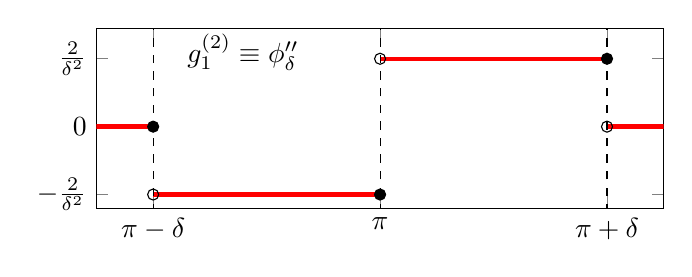
\begin{tikzpicture}
\begin{axis}[
    width=250pt,height=110pt,
    xmin=pi-0.5,xmax=pi+0.5,
    ymin=-1.2,ymax=1.45,
    samples=50,
    xtick={pi-\dlt, pi, pi+\dlt},
    xticklabels={$\pi - \delta$, $\pi$, $\pi + \delta$},
    ytick={-1, 0, 1},
    yticklabels={$-\frac{2}{\delta^2}$, $0$, $\frac{2}{\delta^2}$},
    grid style={line width=.1pt, draw=gray!10}]

    \addplot[red, ultra thick, domain=0:pi-\dlt] (x, 0);
    \addplot[red, ultra thick, domain=pi+\dlt:4] (x, 0);
    \addplot[red, ultra thick, domain=pi-\dlt:pi] (x, -1);
    \addplot[red, ultra thick, domain=pi:pi+\dlt] (x, 1);

    \draw [dashed] (axis cs:{pi-\dlt},-2) -- (axis cs:{pi-\dlt},2);
    \draw [dashed] (axis cs:{pi},-2) -- (axis cs:{pi},2);
    \draw [dashed] (axis cs:{pi+\dlt},-2) -- (axis cs:{pi+\dlt},2);
    
    \node at (axis cs:2.9,1.1) {$g^{(2)}_1 \equiv \phi''_\delta$};

    \addplot[mark=*] coordinates {(pi-\dlt,0)};
    \addplot[mark=o] coordinates {(pi-\dlt,-1)};
    \addplot[mark=*] coordinates {(pi,-1)};
    \addplot[mark=o] coordinates {(pi,1)};
    \addplot[mark=*] coordinates {(pi+\dlt,1)};
    \addplot[mark=o] coordinates {(pi+\dlt,0)};
\end{axis}
\end{tikzpicture}
\undef\dlt